\chapter{Learning from ideal data\\}
\label{cha:Learning_algorithm}

This chapter is focussing on the implementation of the inverse reinforcement learning idea that is used to learn the different weights in the comfort cost function $\bm{\theta}^T\bm{F}(\bm{r})$
explained in chapter \ref{cha:Literature_study}. The use of ideal data is assumed which means that vehicle model mismatch is avoided by using the same model for learning the weights as generating the data. Thereby is the approximation that comfort of a driver can be modelled by a simple linear relation of features exactly for-filled. Data is generated by choosing a set of weights and generating kinematic vehicle signals by the minimization seen in equation \ref{eq:6}. Perfect learning occurs when the chosen weights used in generating the data are found back.\\

First the non-linear bicycle model with the used parameters is explained. Further on, the concrete used algorithm is discussed. After that a detailed discussion is given about the simulations done. It is worth noting that the learning process discussed, concerns an offline optimization which allows for higher calculations loads because of the absence of binding real time constraints.


\section{Non-linear bicycle model}\label{sec:Vehicle_models}
The free body diagram of the non-linear bicycle model can be seen in figure \ref{fig:bicycle_model}.\\

\begin{figure}[h!]
	\centering
	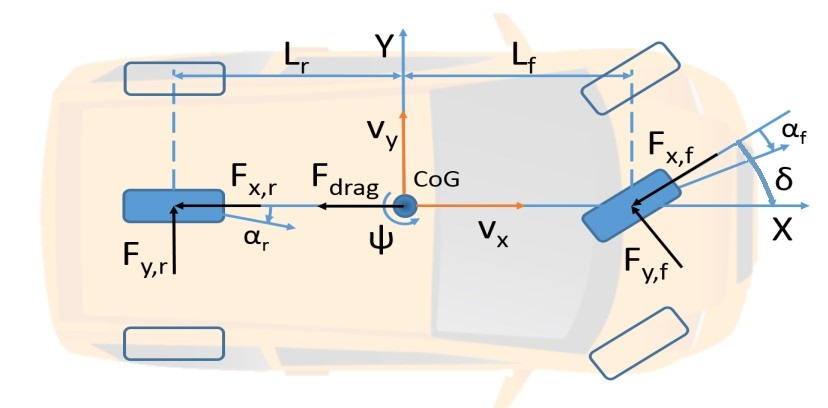
\includegraphics[width=0.5\textwidth]{Bicycle_model_paper.png}
	\caption{Non-linear vehicle bicycle model (Source: \cite{TongDuySon2019}).}
	\label{fig:bicycle_model}
\end{figure}

Two variants of this model are discussed which are differentiated by the smoothness of the controls that can be received. 
\begin{enumerate}
	\item	Model has 6 states and 2 inputs: 
	\begin{equation}\label{eq:bicycle_model1}
	\centering
	\bm{X} = 
	\begin{bmatrix}
	x & y & v_x & v_y & \psi & \dot{\psi}
	\end{bmatrix}^{T}
	\; and \; \bm{U} = 
	\begin{bmatrix}
	t_r & \delta
	\end{bmatrix}^{T}
	\end{equation}
	
	\item Model has 10 states and 2 inputs:
	\begin{equation}\label{eq:bicycle_model2}
	\centering
	\bm{X} = 
	\begin{bmatrix}
	x & y & v_x & v_y & \psi & \dot{\psi} & t_r & \delta & a_x & a_y
	\end{bmatrix}^{T}
	\; and \; \bm{U} = 
	\begin{bmatrix}
	\dot{t_r} & \dot{\delta}
	\end{bmatrix}^{T}
	\end{equation}
\end{enumerate}


$x$ and $y$ in the above formulation are the position of the centre of gravity of the car in the global coordinate system. $v_x$ and $v_y$ are the vehicle velocities in the local vehicle frame.$\psi$ is the vehicle yaw angle and $\dot{\psi}$ the yaw rate.  The input vector of \ref{eq:bicycle_model1} consists of the throttle control input $t_r$ and the angle of the front wheel $\delta$. In the more extended bicycle model of \ref{eq:bicycle_model2} throttle and frontwheelangle serve as states. $a_x$ and $a_y$ are the total accelerations of the centre of gravity in the local vehicle frame. The inputs in this second formulation are the first order derivatives of throttle and frontwheelangle.\\

The equations of motion derived and checked in literature \cite{TongDuySon2019} are\footnote{Appendix \ref{app:A} shows the fully worked out jerk equations $j_x$ and $j_y$.} :
\begin{equation}\label{eq:bicycle_model_eqmotion}
\begin{aligned}
\dot{x} = v_x cos(\psi) - v_y sin(\psi)\\
\dot{y} = v_x sin(\psi) + v_y cos(\psi)\\
m \dot{v}_x = F_{x,f} cos(\delta) - F_{y,f} sin(\delta) + F_{x,r} - F_{drag} + m v_y \dot{\psi}\\
m \dot{v}_y = F_{x,f} sin(\delta) + F_{y,f} cos(\delta) + F_{y,r} - m v_x \dot{\psi}\\
\dot{\psi} = \dot{\psi}\\
I_z \ddot{\psi} = L_f (F_{y,f} cos(\delta) + F_{x,f} sin(\delta)) - L_r F_{y,r}\\
\dot{t_r} = \dot{t_r}\\
\dot{\delta} = \dot{\delta}\\
a_{tx} = \dot{v}_x\\
a_{nx} = -v_y\dot{\psi}\\
a_{ty} = \dot{v}_y\\
a_{ny} = v_x\dot{\psi}\\
j_x = \dot{a}_{tx} + \dot{a}_{nx}\\
j_y = \dot{a}_{ty} + \dot{a}_{ny}
\end{aligned}
\end{equation}

The drag force is calculated as:
\begin{equation}\label{eq:bicycle_Fdrag}
\begin{aligned}
F_{drag} = C_{r0} + C_{r1} v_x^2
\end{aligned}
\end{equation},
with $C_{r0}$ the roll resistance and $C_{r1}$ the air drag contributions.\\

To calculate the tyre forces, a linear tyre model is used instead of a more complex non-linear model e.g. Pacejka tire model. The longitudinal tyre forces are calculated as:
\begin{equation}\label{eq:bicycle_Fx}
\begin{aligned}
F_{x,f} = \frac{t_r T_{max}}{2 R_w}\\
F_{x,r} = F_{x, f}
\end{aligned}
\end{equation}

$R_w$ is the wheel radius and $T_{max}$ a measure for the maximum torque the engine is able to supply. Because $F_{x,r} = F_{x, f}$ the longitudinal forces that are induced by the engine is equally distributed between front and rear axle (division by 2 in above equations). The coefficient $t_r$ is the normalised amount of throttle that can be applied and has a value between -1 and 1 (negative for braking). In the bicycle model it is assumed that braking behaves the same as giving a negative amount of throttle.
The lateral tyre forces are calculated based on the tyre slipangles $\alpha_f$ and $\alpha_r$:
\begin{equation}\label{eq:bicycle_slipangle}
\begin{aligned}
\alpha_f = -atan(\frac{\dot{\psi} L_f + v_y}{v_x}) + \delta\\
\alpha_r = atan(\frac{\dot{\psi} L_r - v_y}{v_x})
\end{aligned}
\end{equation},
resulting in:
\begin{equation}\label{eq:bicycle_Fy}
\begin{aligned}
F_{y,f} = 2 K_f \alpha_f\\
F_{y,r} = 2 K_r \alpha_r
\end{aligned}
\end{equation}\\
The use of this linearised lateral tyre model is valid for small lateral accelerations ($a_y <= 4 m/s^2$) and slip angles ($\alpha <= 5^o$) \cite{TongDuySon2019}. It is acceptable to use this approximation model in this thesis as the goal is learn a comfortable and thus smooth lane change manoeuvre. These constraints will also be checked during the section \ref{s:GD_val}.\\

The vehicle model parameters used are given in table \ref{table:vehicel_model_param}. These correspond to common used vehicle parameters as provide by Siemens Digital Industries Software - NVH R\&D engineering department. The $Gsteerfactor$ approximates linearly the relation between the frontwheelangle and the steeringwheelangle turned by the driver by the relation $\delta = \frac{\delta_s}{Gs}$.  

\begin{table}[h]
	\centering
	\begin{tabular}{|p{5cm}|p{2cm}|}
		\hline
		\textbf{Parameter} & \textbf{Value}\\ \hline		
		Vehicle mass $m$ [kg] & 1430\\ \hline
		Moment of inertia $I_z$ [$kgm^2$] & 1300\\ \hline
		Front axle distance $L_f$ [m] & 1.056\\ \hline
		Rear axle distance $L_r$ [m] & 1.344\\ \hline
		Roll resistance coefficient $C_{r0}$ [N] & 0.6\\ \hline
		Air drag coefficient $C_{r1}$ [$\frac{Ns^2}{m^2}$] & 0.1\\ \hline
		Engine torque limit $T_{max}$ [Nm] & 584\\ \hline
		Wheel radius $R_w$ [m] & 0.292\\ \hline
		Lateral front tyre stiffness $K_{f}$ [N] & 41850.85\\ \hline
		Lateral rear tyre stiffness $K_{r}$ [N] & 51175.78\\ \hline
		Gsteeringfactor $Gs$ [-] &16.96 \\ \hline
		
	\end{tabular}
	\caption{Used vehicle model parameters.}
	\label{table:vehicel_model_param}
\end{table}
\newpage
\section{Formulation of the algorithm} \label{s:learning_alg}
The goal of the learning algorithm is to learn the weights $\bm{\theta}$ in the pre-defined comfort objective function: $\bm{\theta}^T\bm{F}(\bm{r})$. The features that are the entries of the feature vector $\bm{F}(\bm{r})$ capture a notion of comfort felled by the driver. Based on the literature study conducted in Chapter \ref{cha:Literature_study} and paper \cite{Kuderer2015a}, the amount of discomfort can be modelled by the features discussed in \ref{s:obj} during timespan $T$ of the maneuver. The scenario of a lane change on a highway is chosen. The time horizon where over the minimization of the comfort objective is itself also an optimization variable  $T$. The simulations done in this thesis were performed on a notebook provided by Siemens with Intel Core i7-7920HQ CPU @ 3.10GHz and 32 GB of RAM memory.\\


\subsection{Flow of the algorithm}
The goal of the learning algorithm is to output weights that when applied in the objective $\bm{\theta}^T\bm{F}(\bm{r})$, generate feature vector  $\bm{F(\bm{r})}$ that are the best possible fit with the observed feature vector. Without a vehicle mismatch a match of feature values will directly induce a good match of the kinematic signals as is extensively discussed in section \ref{s:ID_results}. This means that similarity between the observed path and the one that follows from minimizing the objective $\bm{\theta}^T\bm{F}(\bm{r})$ for chosen weights, is quantified by the difference between the feature values of the observed path and the obtained one. The flow of a single data set learning algorithm can be seen in Figure \ref{fig:basic learning}. The path that is expected to be produced by the driver is the path that is felt the most comfortable and equals $\bm{r}_{expected} =  \underset{\bm{r}}{\argmin} \hspace{1mm}  \bm{\theta}^T\cdot \bm{F}(\bm{r})$

\begin{figure}[h!]
	\centering
	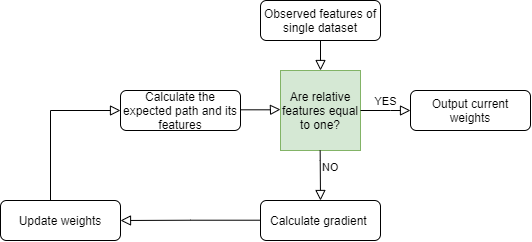
\includegraphics[width=1.0\textwidth]{basic_learning.png}
	\caption{Basic flow of the reinforced learning algorithm.}
	\label{fig:basic learning}
\end{figure}

The learning is started by guessing a set of weights e.g. all equal to one. Equation \ref{eq:6} is minimized in order to generate an expected path for these weights. From this calculated path, features for the observation and the calculated path from optimization \ref{eq:6},further addressed as learned features, can be retrieved by using the definition of the features discussed in \ref{s:obj}.From this the relative features $f_{rel,i}$ are calculated by dividing the learned features by the observed features. A perfect match is acquired when the division equals one and the learning algorithm is terminated. The tolerance on convergence towards one, is chosen during this chapter equal to $10^{-3}$.  

While no convergence takes place the weights are updated, making use of the RPROP algorithm explained in Chapter \ref{cha:Literature_study}. In order to apply the RPROP method only the sign of the gradient is used which means that the size of the gradient is decoupled from the update value of the weights. The gradient is given by $\pdv{\bm{F}}{\bm{\theta}} = \bm{F}_{obs} - \bm{F}(\bm{r}_{expected})$  and the update of the weight is achieved by applying the gradient method according to $\bm{\theta}^{k+1} = \bm{\theta}^{k} - |\Delta \theta^{k}|sign( \pdv{\bm{F}}{\bm{\theta}}^k )$ where $\Delta \theta^{k}$ is calculated according section \ref{s:RPROP}. If follows that the weight $\theta_i$ is decreased if $f_{obs,i}>f_{i}(\bm{r_{exptected}})$ and increased when $f_{obs,i}<f_{i}(\bm{r}_{exptected})$. the new weights can be used in the minimization of the comfort objective for a set of weights given by \ref{eq:6}. Next a more detailed description of how this is done is given by \ref{opt:basic_opti_w} which uses as vehicle model \ref{eq:bicycle_model2}. \\

\begin{equation}\label{opt:basic_opti_w}
\begin{aligned}
\min_{\bm{X}(.),\bm{U}(.), T} \quad &  \bm{\theta}^T\bm{F}(\bm{X},\bm{U}, T) \\
\textrm{s.t.} \quad & \bm{X}^{k+1} = I(\bm{X}^{k}, \bm{U}^{k}) & k = [0,\cdots, N-1]\\
& \bm{X}^{0}(1:8)= \bm{X}_{intitial} \\
& T \leq T_{limit}\\
& \bm{F}(\bm{X}^{k}) \geq 0	& k = [0,\cdots, N]\\
& \bm{G}(\bm{U}^{k}) \geq 0	& k = [0,\cdots, N-1]\\
& \bm{H}(\bm{X}^{k}) = 0	& k = [0,\cdots, N]\\
& \bm{X}^{k}\in \mathbb{R}^{6x1}  & k = [0,\cdots, N]\\
& \bm{U}^{k}\in \mathbb{R}^{2x1} \hspace{3 mm} & k = [0,\cdots, N-1]\\
& T \in \mathbb{R},\hspace{3 mm} N,i,l \in \mathbb{N}
\end{aligned}
\end{equation}

Where $\bm{X} \in \mathbb{R}^{10xN+1}$ and $\bm{U}\in \mathbb{R}^{2xN}$ contain respectively the states and controls  \ref{eq:bicycle_model2} during the maneuver, complemented with the time of the maneuver $T$. In order to discretize time, a multiple shooting approach is adopted as is explained in section \ref{s:time_dis}. The amount of integration intervals $N$ is chosen equal to $1000$ and is the same as the amount of control intervals in order to go from the initial state towards the end state. With this a sampling time of $0.025 \hspace{1mm}s$ is obtained as is discussed in section \ref{s:GD_val}.  Inside the function $I$ the Runge-Kutta time integration method is embedded in order to connect different states over time when a certain control is applied for $\Delta T$. Here the equations of motion \ref{eq:bicycle_model_eqmotion} are inputted in the optimization because to perform the integration, derivatives of the vehicle states are used. The time discretization used is can be categorized as a direct method and a multiple shooting approach is used which means that at every time instance a new set of state optimization variables is introduced as is explained in section \ref{s:time_dis}. The path constraint vectors $\bm{F} \in \mathbb{R}^{L_1x1}$ and $\bm{G} \in \mathbb{R}^{L_2x1}$ demarcate together with the equality constraint vectors $\bm{H} \in \mathbb{R}^{Q_1x1}$ and $\bm{J} \in \mathbb{R}^{Q_2x1}$ the feasible area of the solutions for $\bm{X}$, $\bm{U}$ and $T$. An overview of these constraints is given by equations \ref{eq:F}, \ref{eq:G} and \ref{eq:H}.

\begin{equation}\label{eq:F}
\bm{F} =
\begin{Bmatrix}
-\frac{Width\hspace{1mm}Lane}{2} \leq y^k \leq \frac{3\cdot Width\hspace{1mm}Lane}{2}, & k = [0,\cdots, N] \\
0 \leq x^k, & k = [0,\cdots, N] \\
-\frac{\pi\cdot 150}{180 Gs} \leq \psi^k \leq \frac{\pi\cdot 150}{180 Gs}, & k = [0,\cdots, N] 

\end{Bmatrix}
\end{equation}\\

\begin{equation}\label{eq:G}
\bm{G} =
\begin{Bmatrix}
-1 \leq t_r^k \leq 1, & k = [0,\cdots, N-1]
\end{Bmatrix}
\end{equation}\\

It is not necessary to introduce physical vehicle limits because these are present as soft constraints in the comfort objective $\bm{\theta}^T\bm{F}(\bm{X},\bm{U}, T)$.

\begin{equation}\label{eq:H}
\bm{H} =
\begin{Bmatrix}
y^N = Width\hspace{1mm}Lane \\ \vspace{1mm}
vy^N = 0 \\\vspace{1mm}
\psi^N = 0 \\\vspace{1mm}
\dot{\psi}^N = 0 \\\vspace{1mm}
\delta^N = 0 

\end{Bmatrix}
\end{equation}\\

The constraints displayed in $\bm{H}$ make sure that at the end of the lane change the slipangles in the tires and the steerwheelangle are zero. From \ref{eq:bicycle_model_eqmotion} this induces that the lateral velocity and acceleration and yaw acceleration also becomes zero and the lane change is completed. $y^N$ makes sure that the wanted lateral distance is covered. This distance can be calculated from the start position of the vehicle in its lane and the width of the lane in order to end up at the centreline of the desired lane. \\ At the start of the lane change straight driving at constant longitudinal speed is assumed. To obtain this, the constraints of \ref{eq:X0} are used. No constraints for accelerations are needed because this would give a redundancy due to the other initial states in combination with the motion equations \ref{eq:bicycle_model_eqmotion}. In \ref{eq:X0} all initial states are zero excepts for the initial speed $v_{x,start}$ and $t_{r,start}$. The amount of throttle at the start of the lane change is chosen to overcome the aerodynamic drag without accelerating. This is given by $t_r^0 = \frac{(C_{r0}+C_{r1}v_{start}^2)r_w}{T_{max}}$. Therefore it can be concluded that the parameters that distinguish different lane changes are $v_{x,start}$ and $Width\hspace{1mm}Lane$. This is exploited when generating different ideal lane change datasets. 
\begin{equation}\label{eq:X0}
\bm{X}_{initial} =
\begin{bmatrix}
 x_{start}\\ 
 y_{start}\\
 v_{x,start}\\
 v_{y,start}\\
 \psi_{start}\\
 \dot{\psi}_{start}\\
 t_{r,start}\\
 \delta_{start}\\

\end{bmatrix}
\end{equation}\\


% discuss time limit is chosen equal to 25 s.
The time limit constraint in \ref{opt:basic_opti_w} is needed in order to demarcate the optimization solution space. When set it has to take two conflicting criteria. It has to be chosen large enough in order to have a minor influence introduced by this constraint. Secondly it has to be taken small enough in order to preserve good conditions for the numerical integration performed in $\bm{F}(\bm{X},\bm{U}, T)$. This is because the number of optimization points $N+1$ is fixed which means that a larger time limit will give a coarser time discretization. In order to serve these conditions time limit is set in this thesis on $25 s$. This choice is validated in section \ref{s:GD_val}. It is worth noting that with the removal of the time limit constraint the optimized comfortable lane change takes around $160 \hspace{1mm}$. This is not an realistic results because the objective will, as previously explained, not have good numerical properties.\\ 

In order to solve \ref{opt:basic_opti_w} an initial guess is needed for the longitudinal velocity in order to avoid the emergence of an invalid number. The default initial guess used in the CasADi software is an all zero vector. As can be seen in \ref{eq:bicycle_slipangle} this would give a division by zero. \\
To further enhance the solving speed of \ref{opt:basic_opti_w} also initial guesses are given for the other vehicle states and additionally the controls. To do this, a feasible solution of the non-linear bicycle model for a lane change is needed. Therefore the initial guesses for $\bm{X}, \bm{U} \;and\; T$ are taken from the observed ideal data. \\

Another initial guess that speeds up the solving time of the IPOPT solver, is setting the initial guess of the lambda multipliers internally equal to the ones found during the previous call of \ref{opt:basic_opti_w} during the loop visualized by figure \ref{fig:basic learning}. \\

The solver used to calculate the states and control signals in \ref{opt:basic_opti_w} is the interior point solver IPOPT which is an open source solver. The idea behind it is to smoothing the KKT conditions and transform it to a smooth root finding problem. \cite{Panos_opti} Because IPOPT is a interior boundary method, a feasible initial guess is needed. Every time that the expected path has to be calculated as is visualised in flow diagram \ref{fig:basic learning}, the optimization \ref{opt:basic_opti_w} is performed with as initial guess the observed maneuver.\\

The time needed by the CPU in order to calculate the expected path for a certain set of weights and thus solving \ref{opt:basic_opti_w} takes around $5\hspace{1mm}s$ (python implementation) when a timelimit of $30$ seconds and N equal to $1000$ is chosen. 


\subsection{Objective function}\label{s:obj}
The objective function used in \ref{opt:basic_opti_w} has to contain comfort felt by the driver and is based on the literature study displayed in section \ref{s:comfort_parameters}. The choice made in how to define the different features is important because it sets the fixed framework where the weights serve as parameters that steer the learning process towards a better match with the observations. It can be expected that the linear relation of features given by $\bm{F}(\bm{r})$ will serve as an approximation for the real, more complex comfort objective of a human drive. As is showed in \cite{Kuderer2015a} this linear approximation of features can already capture  the main trends that contribute to an comfortable maneuver experience. As is suggested in \cite{Kuderer2015a} the feature framework that is further discussed in this section, can be validated and adjusted based on an user study in order to better match real driver observations. \\

When ideal data is used the observations are generated based on a known underlying comfort objective with known weights and feature framework. This permits the validation of the objective learning method discussed in this thesis. The remaining part of this section will discus the feature framework used in this thesis.\\


\begin{equation}\label{eq:obj}
discomfort = \theta_1 \cdot f_1 +\theta_2 \cdot f_2 +\theta_3 \cdot f_3 +\theta_4 \cdot f_4 +\theta_5 \cdot f_5 +\theta_6 \cdot f_6 \\
\end{equation}
\[	f_i, \theta_i \in \mathbb{R} \hspace{5mm}
i \in \mathbb{N}\]\\


\textit{Feature 1: longitudinal acceleration}
\begin{equation}\label{eq:flong_acc}
f_{1}:\bm{r}\xrightarrow{}f_1(\bm{r})=\int_{0}^{T}a_{x,total}^{2}(t) dt
\end{equation}
Feature one is assessing the amount of discomfort by integrating the total longitudinal acceleration in the local axis. The local axis are fixed to the centre of gravity of the vehicle as can be seen in Figure \ref{fig:bicycle_model}. The total longitudinal acceleration  $a_{x,total} $ is the sum of  $ a_{x,tangential}$ and $a_{x,normal}$ as described in \ref{eq:bicycle_model_eqmotion}. \\

\textit{Feature 2: lateral acceleration}
\begin{equation}\label{eq:flat_acc}
f_{2}:\bm{r}\xrightarrow{}f_2(\bm{r})=\int_{0}^{T}a_{y,total}^{2}(t) dt
\end{equation}
Feature two is assessing the amount of discomfort by integrating the total lateral acceleration in the local axis. The total lateral acceleration  $a_{y,total} $ is the sum of  $ a_{x,tangential}$ and $a_{x,normal}$ as described in \ref{eq:bicycle_model_eqmotion}.\\

\textit{Feature 3: longitudinal jerk}
\begin{equation}\label{eq:flong_jerk}
f_{3}:\bm{r}\xrightarrow{}f_3(\bm{r})=\int_{0}^{T}j_x^{2}(t) dt
\end{equation}
Feature three is assessing the amount of comfort by integrating the total change of longitudinal acceleration during the followed path. \\

\textit{Feature 4: lateral jerk}
\begin{equation}\label{eq:flat_jerk}
f_{4}:\bm{r}\xrightarrow{}f_4(\bm{r})=\int_{0}^{T}j_y^{2}(t) dt
\end{equation}
Feature four is assessing the amount of comfort by integrating the total change of lateral acceleration during the followed path. \\

\textit{Feature 5: desired speed}
\begin{equation}\label{eq:des_speed}
f_{5}:\bm{r}\xrightarrow{}f_5(\bm{r})=\int_{0}^{T}(v_{des}-v_x)^2 dt
\end{equation}
$v_{des}$ is assumed to be a constant value and set equal to the start velocity just before the lane change.\\

\textit{Feature 6: desired lane change}
\begin{equation}\label{eq:des_lane_change}
f_{6}:\bm{r}\xrightarrow{}f_6(\bm{r})=\int_{0}^{T}(y_{lane\_change}-y)^2 dt
\end{equation}

$y_{des}$ is a constant and is the desired lateral distance completed after the lane change. If the vehicle reaches faster its desired lateral displacement this is perceived as a good responds and is interpreted as comfort of the driver as is discussed in section \ref{s:comfort_parameters}.
\\


In order to implement the above defined integrals in the objective function of \ref{opt:basic_opti_w} discretization is needed. For this the Crank-Nicolson numerical integration is used as is shown in \ref{eq:CN} for feature $f_i$. 
\begin{subequations}\label{eq:CN}
	\begin{equation}
	\int_{f_i(t^n)}^{f_i(t^{n+1})}df_i=\int_{t^n}^{t^{n+1}} I(t) \cdot dt	
	\end{equation}
	\begin{equation}
	f_i^{n+1} -f_i^{n} = \frac{1}{2}\frac{I(t^{n+1})+I(t^n)}{\Delta T}
	\end{equation}
\end{subequations}\\

To summarize the objectives described by equation \ref{eq:obj} consists out of a set of comfort features that model the amount of discomfort experienced during a maneuver. This is achieved by mapping kinematic signals onto scalar feature values through integration. By finding the driver specific weights $\bm{\theta}$ in \ref{eq:obj} it is possible to model driver preferences between different comfort features. With this information an autonomous vehicle can perform path planning of the most comfortable path to do a lane change for a specific driver. As is shortly discussed in Chapter \ref{cha:Literature_study}, the perception of save driving of an autonomous vehicle contributes to the amount of comfort that is experienced during driving. A perception of save driving comprises next to smooth behaviour also distances between other road agents. However features that consider the environment are not taken into account in \ref{eq:obj} but this can be done if data of the position of other vehicles during the maneuver is available. Paper \cite{Kuderer2015a} gives some suggestions showed by equations \ref{eq:comfort_feature} and  \ref{eq:lane_d}.  

\begin{equation}\label{eq:comfort_feature}
f_d= \sum_{k = 1}^{L}\int_{0}^{T}\frac{1}{(x_{o,k}(t)-x)^2+(y_{o,k}(t)-y)^2}\cdot dt
\end{equation}
\[L \in \mathbb{N}\]

With $[x_o,y_o]_k$ the position of the closest point of a different vehicle and $L$ the total amount of vehicles in the nearby area.\\

Not only the bird's eye view distance between two different vehicles plays a role, but also the following distance of vehicle in the same lane is important. This can be modelled as suggested by \cite{Kuderer2015a}:  

\begin{equation}\label{eq:lane_d}
f_d= \int_{0}^{T} max(0,\hat{d}-d(t))\cdot dt
\end{equation}


The desired following distance $\hat{d}$ can be calculated based on the stopping distance of the vehicle when driving on a certain longitudinal velocity. \\

An other assumption that is not discussed in this thesis is the time limit to finish a maneuver. In a real life application however this limit often influences the maneuver. After the weights are identified, the most comfortable path in a limited time span can be planned for a specific driver. 

\subsubsection{Normalization factors} \label{s:norm}
In order to reduce the effect of order of size given by the units in the objective discussed in section \ref{s:obj}, a normalization of the features is used. The kinematic signals of an example lane change are produced and the same features that are used in the objective function are calculated from it. These will be the normalization factors. Then the objective function is divided by the corresponding normalization factor which means that a feature that inherently gives a small feature value, will be divided by a small value and the other way around, an inherently large feature value will be divided by a large value. Table \ref{table:norm} gives an overview of the lane change normalization factors used in this chapter. 


%$ \bigl[ \begin{smallmatrix} 4,&5,&6,&1,&2\end{smallmatrix}\bigr]$
\begin{table}[h!]\label{table:norm}
  \centering
  \begin{tabular}{@{}lr@{}} 
    Normalization factor    & Value\\ \midrule
    Nr.1      & 0.0073\\
    Nr.2          & 2.64\\
    Nr.3 	   & 0.0073\\
    Nr.4       & 11.28\\
    Nr.5       & 0.047\\
    Nr.6  & 17.14\\ \bottomrule
  \end{tabular}
  \caption{Overview of  normalization factors.}
\end{table}


\section{Ideal data} \label{s:GD}
\subsection{Generation}
As mentioned above the term 'ideal data' concerns data that is generated with a non-linear bicycle model and exactly fulfils the assumption that the observations are minimizing an underlying comfort objective. More over the discomfort objective is the same as the one used in the learning algorithm which means that the generated path is a solution of the objective function discussed in section \ref{s:obj} for weights $\bm{\theta}$ known in advance. Because that the observations are using the same feature frame as the learning algorithm and the absence of vehicle model mismatch, weights can be learned that accurately explain the observations. This is translated in a accurate matching of the feature values discussed in \ref{s:obj}. Because beforehand it is know what the weights should be in \ref{eq:obj}, the ideal data can serve as a validation of the learning algorithm discussed in section \ref{s:learning_alg}.\\


The relative weights $\theta_{r,i} = \frac{\theta_{abs,i}}{norm_i}$ chosen are $ \bigl[ \begin{smallmatrix} 4,&5,&1,&6,&1,&2\end{smallmatrix}\bigr]$, which gives as absolute weights  $ \bigl[ \begin{smallmatrix} 549.75, &1.90, &137.44  ,&0.53,  &21.43, &0.12\end{smallmatrix}\bigr]$ when the normalization of \ref{s:norm} is taken into account. The objective that is used in \ref{opt:basic_opti_w} and outputs the ideal data is given by \ref{eq:obj_ideal_data}. 
\begin{equation}\label{eq:obj_ideal_data}
discomfort = \frac{4}{0.0073} \cdot f_1 +\frac{5}{2.64} \cdot f_2 +\frac{6}{11.28} \cdot f_3 +\frac{1}{0.047} \cdot f_4 +\frac{2}{17.14} \cdot f_5 \\
\end{equation}
\[	f_i \in \mathbb{R}, \hspace{1mm}
i \in \mathbb{N}\]\\

Because of the normalization the relative weights will quantify the trade-offs between different comfort features without the disturbance of units used. Aside of this it allows to learn weights faster, because of the absence of big size differences that are present in the absolute weights. During the learning loop (Figure \ref{fig:basic learning}) the weights are set on a maximum of $1$. When the absolute weights are learned instead of the relative ones, this would cause a substantially higher amount of iterations.  When multiple ideal data sets have to be generated in order to serve as observations, the initial speed and width of the lateral distance are varied.\\

\subsection{Validation} \label{s:GD_val}
In this section the results of the generated ideal data are discussed. There is being look at the influence of the initial guess, amount of optimization points and choice of time limit on the generated data.
\subsubsection{Initial guess}

To determine if the generated data is a local solution of the optimization of \ref{eq:obj_ideal_data}, two different initial guesses are used whereof the obtained data feature values are summarized in table \ref{tab:GD_local_test}. In order to calculate the features, time limit is set on $30\hspace{1mm}s$ and N on $1000$. From the results it can be concluded that the optimized features are not a local solution. In table \ref{tab:GD_local_test}  V is the initial speed and L the lateral distance of the lane change used as initial guess. During the learing of the weights as described by Figure \ref{fig:basic learning} the initial guess is set equal to the observed data. 

\begin{table}[h!]
	\centering
	\begin{tabular}{@{}llr@{}} \toprule
		Feature Value    & V22.22 - L3.47 & V25.00 - L6.94\\ \midrule
		Nr.1       & 6.83e-8   & 6.83e-8 \\
		Nr.2       & 0.37        & 0.37  \\
		Nr.3       & 1.77e-7     & 1.77e-7 \\
		Nr.4       & 0.57    & 0.57  \\
		Nr.5       & 1.98e-6     & 1.98e-6 \\
		Nr.6       & 30.94      & 30.94\\ \bottomrule
	\end{tabular}
	\caption{This table shows the retrieved feature values using different initial guesses in \ref{opt:basic_opti_w}.}
	\label{tab:GD_local_test}
\end{table}

\subsubsection{Time limit}
In order to check the dependency of the generated data on the chosen $T_{limit}$ constraint in \ref{opt:basic_opti_w}, data is generated for an lane change with N, the amount of control points equal to $1000$, initial velocity equal to $80 \hspace{1 mm} \frac{km}{h}$, a desired lateral displacement of $3.47\hspace{1mm}m$ and a varying $T_{limit}$ constraint as indicated in table \ref{tab:GD_time_limit}. Figures that  show what the difference in the feature means for the different kinematic signals of the vehicle during a lane change, can be consulted in Appendix \ref{app:B}

\begin{table}[h!]
	\centering
	\begin{tabular}{@{}llllr@{}} \toprule
		Feature Value    & 20 s  & 50 s      & 100 s\\ \midrule
		Nr.1       & 3.66e-8     & 1.13e-7   & 2.04e-7\\
		Nr.2       & 0.37        & 0.38      & 0.38\\
		Nr.3       & 1.13e-7     & 3.98e-7   & 1.56e-6 \\
		Nr.4       & 0.58        & 0.57      & 0.54\\
		Nr.5       & 1.72e-6     & 2.27e-6   & 3.16e-6\\
		Nr.6       & 31.05       & 30.74     & 30.42\\ \bottomrule
	\end{tabular}
	\caption{This table shows the retrieved feature values using different time limits in \ref{opt:basic_opti_w}.}
	\label{tab:GD_time_limit}
\end{table}
Looking at even greater time limits is not desirable because beyond a time limit of $100 \hspace{1mm}s$, the time discretization gets larger than $0.1\hspace{1mm}s$ for N equal to $1000$ and thus more unreliable.\\

From the result of table \ref{tab:GD_time_limit} it can be concluded that the influence of the manually setting of the time limit in \ref{opt:basic_opti_w} can be neglected. 




\subsubsection{Amount of optimization points}
The test carried out to investigate the dependence of resulting features values uses the same parameters as described in the previous section but fixes the time limit on $30\hspace{1mm}s$ and varies N over $500$, $1000$ and $1500$ points. The results are shown in table \ref{tab:GD_N} whereof it follows that a choice of N equal to $1000$ is justified considering the small difference of the obtained features when N is equal to $1500$ and a lower calculation load.

\begin{table}[h!]
	\centering
	\begin{tabular}{@{}llllr@{}} \toprule
		Feature Value    & 500  & 1000      & 1500 s\\ \midrule
		Nr.1       & 9.42e-8     & 6.63e-8   & 6.45e-8\\
		Nr.2       & 0.38        & 0.37      & 0.37\\
		Nr.3       & 5.61e-7     & 1.77e-7   & 1.11e-7 \\
		Nr.4       & 0.56        & 0.57      & 0.58\\
		Nr.5       & 2.50e-6     & 1.98e-6   & 1.85e-6\\
		Nr.6       & 30.66       & 30.94     & 31.05\\ \bottomrule
	\end{tabular}
	\caption{This table shows the retrieved feature values using different amount of control point N in \ref{opt:basic_opti_w}.}
	\label{tab:GD_N}
\end{table}


\subsubsection{Linear tire model}
In this section it is checked if the conditions to use a linearised lateral tire model is valid. In literature \cite{TongDuySon2019} it was found that this is the case when there are small lateral accelerations ($a_y <= 4 m/s^2$) and slip angles ($\alpha <= 5^o$) during the maneuver. Figure \ref{fig:lat_acc_val} gives the total lateral acceleration during a lane change maneuver that moves around two lanes or an estimated lateral distance of $6.94 m$. Figure \ref{fig:slipangle_val} shows the slip angle during this maneuver. From the graphs it can be concluded that the linearisation of the lateral tire forces is valid and there is no need for a more complex tyre model in \ref{opt:basic_opti_w}.  Both resulting figures are generated with complex vehicle model discussed in chapter \ref{cha:Tracking_MPC}.

 \begin{figure}[h!]
	\centering
	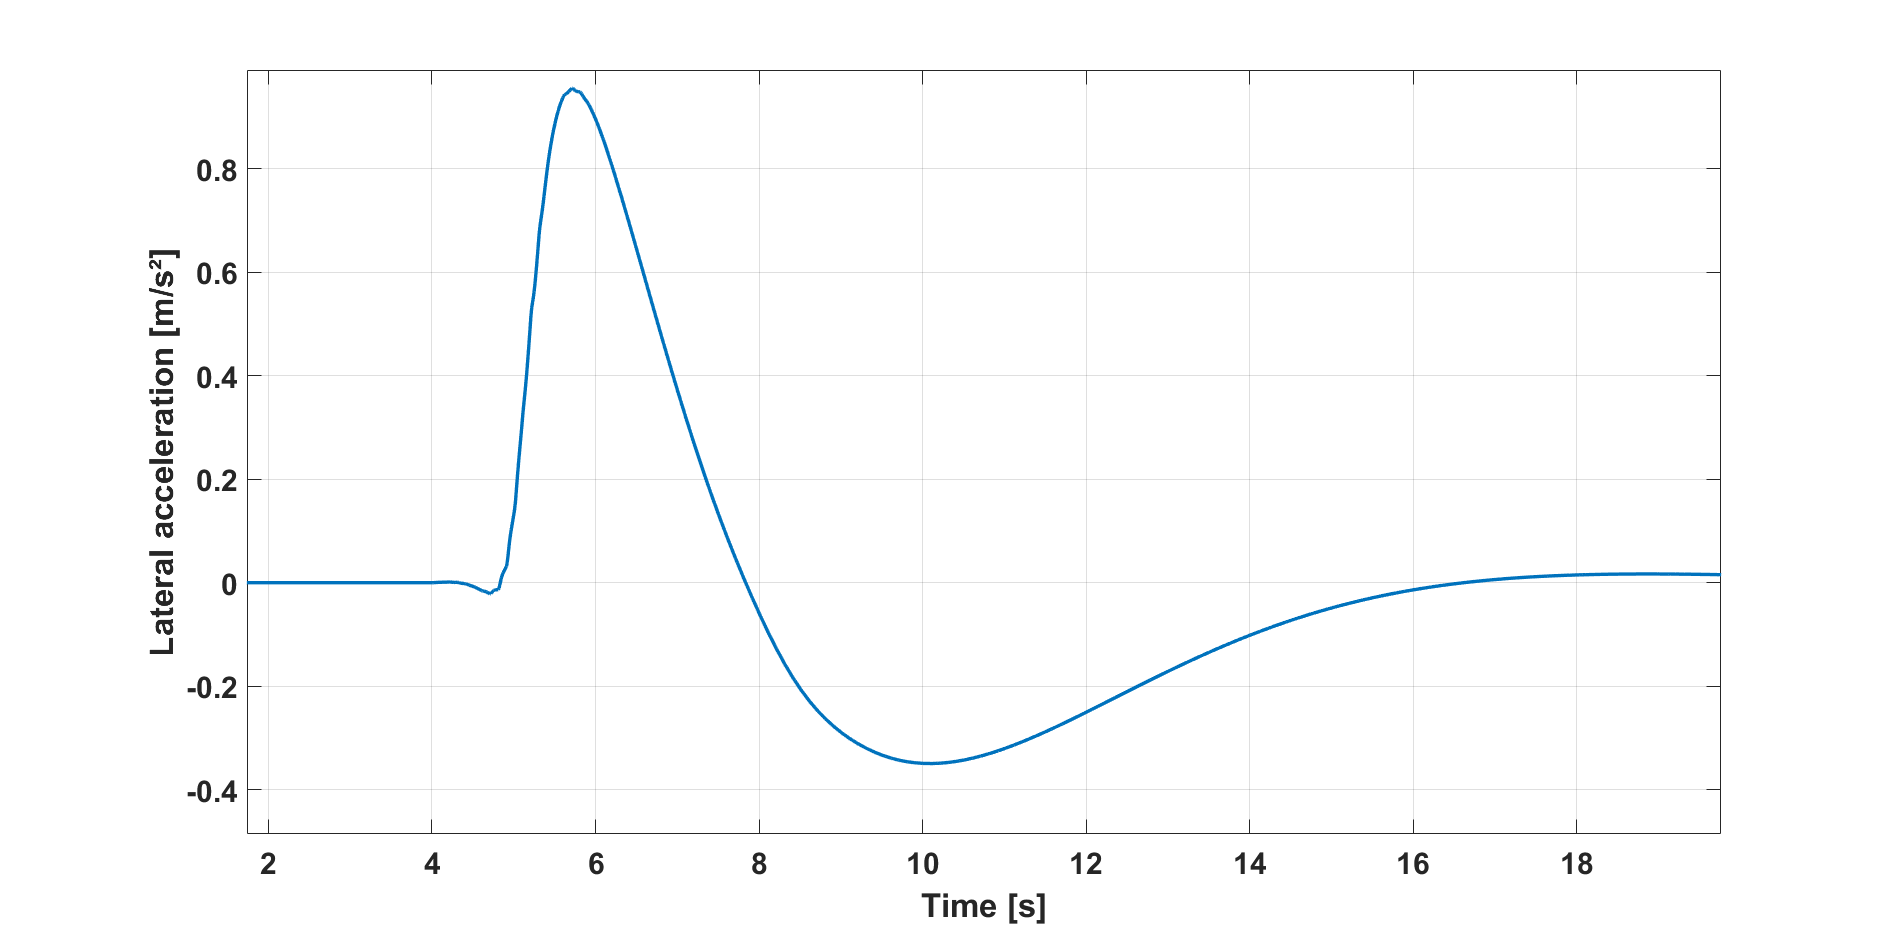
\includegraphics[width=1.0\textwidth]{lat_acc.png}
	\caption{Lateral acceleration during a lane change $V_0: 25.00 \frac{m}{s}$ and $L:6.94 m$ generated with the amesim model.}
	\label{fig:lat_acc_val}
\end{figure}

 \begin{figure}[h!]
	\centering
	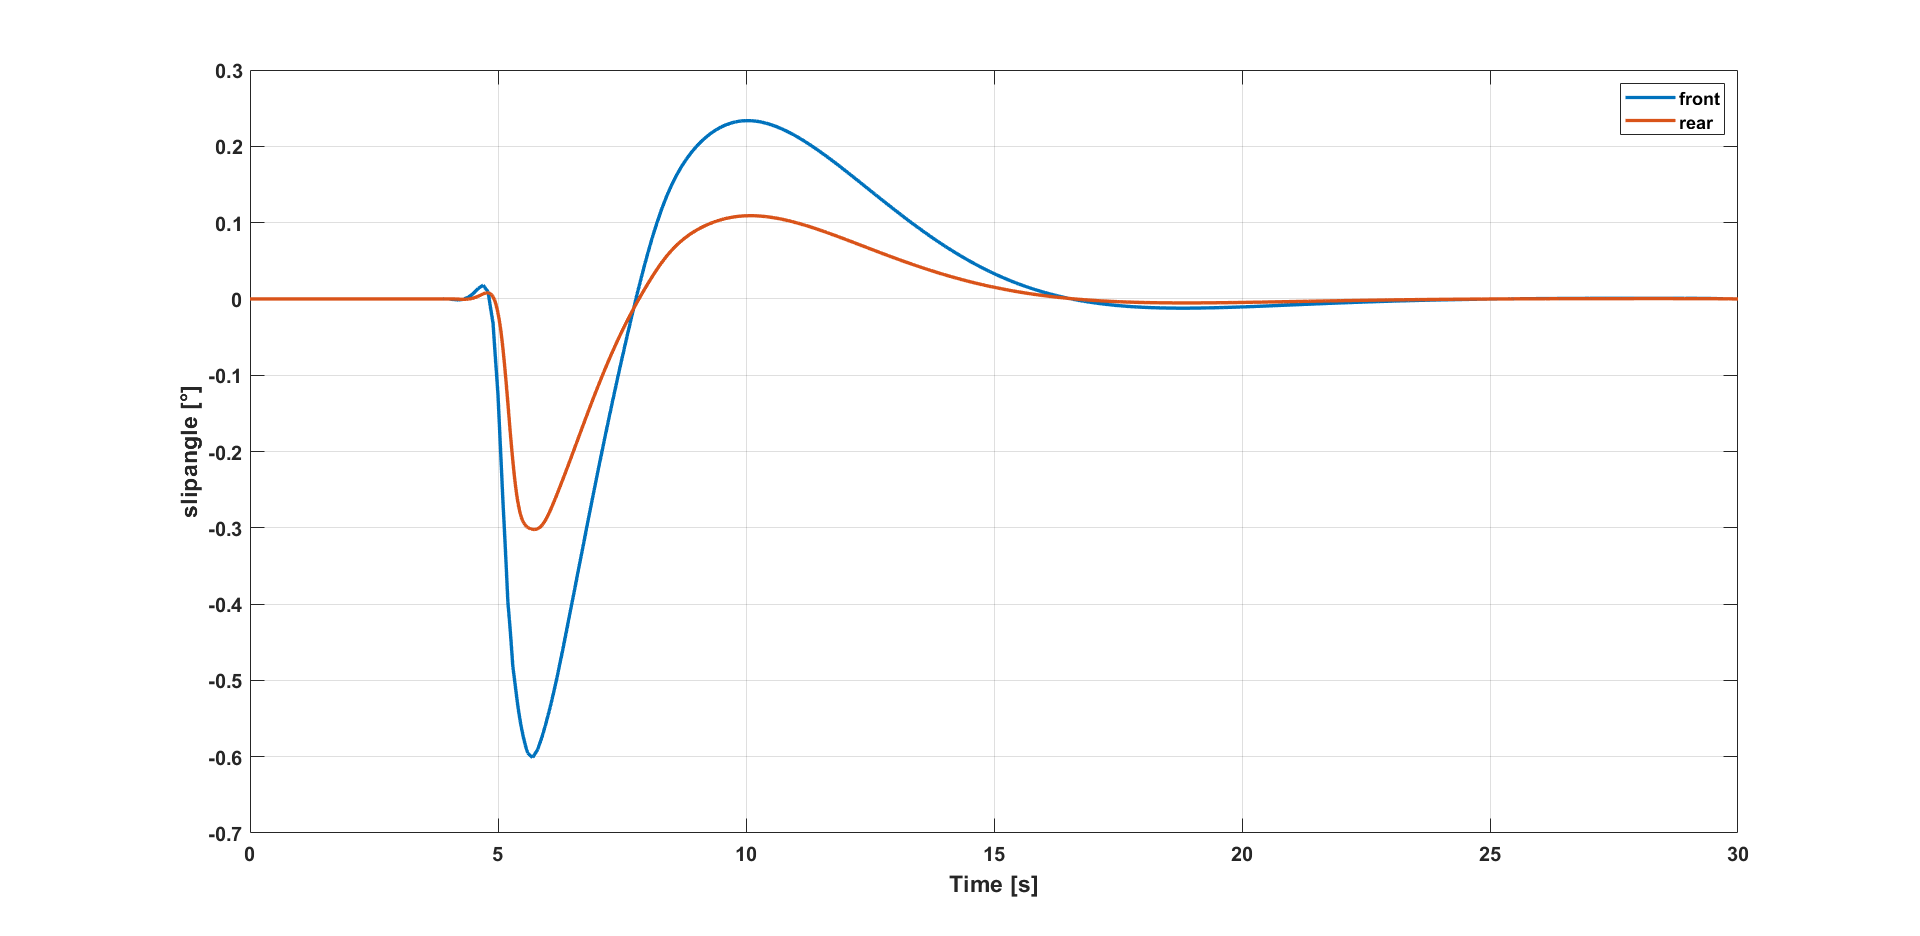
\includegraphics[width=1.0\textwidth]{slipangle.png}
	\caption{Slipangle during lane change $V_0: 25.00 \frac{m}{s}$ and $L:6.94 m$ generated with the amesim model.(bleu:front,red:rear)}
	\label{fig:slipangle_val}
\end{figure}

\subsubsection{Numerical vs Analytical approach}
In section \ref{sec:Vehicle_models} about the non-linear bicycle model, two different variants were described by equations \ref{eq:bicycle_model1} and \ref{eq:bicycle_model2}. Variant one has only 6 states and the accelerations and jerks in the objective function \ref{eq:obj} are calculated by making use of numerical differentiation described by equations \ref{eq:diff}. Variant two on the other hand uses the total accelerations as direct states in the vehicle model and uses an formulation of the jerk described in appendix \ref{app:A}.

\begin{subequations}\label{eq:diff}
\begin{equation}
\pdv{\phi}{t} = \frac{\phi(i+1)-\phi(i-1)}{2\Delta t}
\end{equation}
\begin{equation}
\pdv[2]{\phi}{t} = \frac{\phi(i+1)\phi(i)+\phi(i-1)}{\Delta t^2}
\end{equation}
\end{subequations}

In order to validate the two approaches the generated lateral jerk signals are compared. 

\begin{figure}[h!]
	\centering
	\begin{minipage}{.5\textwidth}
		\centering
		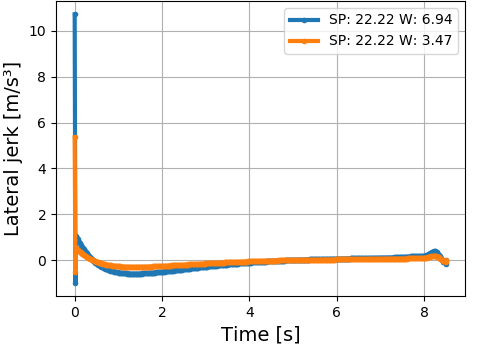
\includegraphics[width=0.9\linewidth]{jerk_num.png}
%		\captionof{figure}{Lateral jerk using \ref{eq:diff}.}
		\label{fig:num}
	\end{minipage}%
	\begin{minipage}{.5\textwidth}
		\centering
		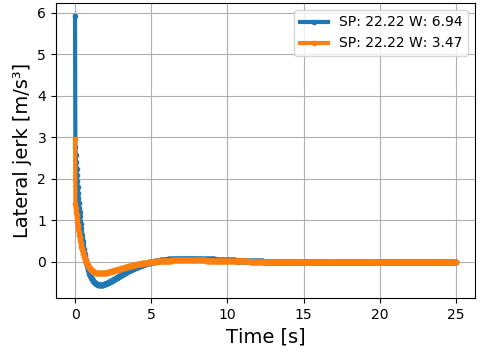
\includegraphics[width=0.9\linewidth]{jerk_ana.png}
%		\captionof{figure}{Lateral jerk using appendix \ref{app:A} .}
		\label{fig:ana}
	\end{minipage}
	\caption{A comparison between the numerical jerk (left) based on \ref{eq:diff} and \ref{eq:bicycle_model1} and the analytical jerk (right) based on appendix \ref{app:A} and \ref{eq:bicycle_model2}. }
\end{figure}

It is clear that the analytical formulation (right figure)  of the jerk gives more smooth results and less high peaks which is also seen in the more complex vehicle that is discussed in chapter \ref{cha:Tracking_MPC}. Therefore the analytical formulation approaches reality better. An other way to see this is that the analytical formulation contains more information about the vehicle, because the numerical equation of \ref{eq:diff} are approximations of the equations shown in appendix \ref{app:A}. 

\subsubsection{Feature values} \label{s:fv_val}
% Steeds dezelfde als enkel horizontale init speed verandert --> zelfde gewichten zullen geleerd worden aangezien enkel de lateral featues bijdragen. 
In the above tables it can be seen that the first, third and fifth features concerning longitudinal behaviour of the vehicle are very small. This means that during a lane change these features have a low influence. It can be expected that for the values with an order of size in computer accuracy, it becomes hard to accurately learn weights that generate feature values that match with these small values. This will be further discussed in \ref{label}.\\% A suggested solution for this is the use of different features or an different maneuver. Scaling in the calculation of the gradient doesn't help. RPROP update is independent of the order of size of the gradient. 

An other interesting thing to note about the ideal data generated features is that when the initial speed of the lane change is varied and the desired lateral displacement stays the same ($3.47m$ or $6.97m$), because of the small longitudinal features values the data features found are quasi identical.

\subsubsection{Conclusion}
From the above results it the influence of the choice of taking the time limit constraint equal to $30 \hspace{1mm}s$ and the amount of control points equal to $1000$ further on in this thesis, has been validated. Next it is shown that it is justified to use a linearised tire model. Afterwards an numerical and analytical formulation to model the total accelerations and jerk is discussed. Finally the resulting feature values of the ideal data are shortly look into. 

\textbf{write something about small longitudinal features and resulting bad weight learning.}
\section{Ideal lane change data learning results} \label{s:ID_results}
In this section the results of the learning algorithm which makes use of ideal data is discussed. The first result discussed concerns the learning of a single dataset with $V_0:22.22\hspace{1mm}\frac{m}{s},\hspace{1mm} L:3.47\hspace{1mm}m$. It is known beforehand that the weights used to generate the data are  $\bigl[ \begin{smallmatrix} 4,&5,&1,&6,&1,&2\end{smallmatrix}\bigr]$ and the initial guess of the weights is chosen as an all one vector. The convergence criteria to stop the learning algorithm displayed in Figure \ref{fig:basic learning} is when the maximum amount of iterations equal to $300$ is reached or if the feature values which use the learned weight match accurately the ones of the observed data according to following formula $f_{rel,i} = \frac{f_{calc,i}}{f_{obs,i}} \leq 10^{-3}$. The generated data features that are supposed to be matched in section \ref{s:SDL}, can be seen in table \ref{tab:GD_local_test}. Convergence is reached when the three lateral features, that dominantly define the lane change, are accurately fitted for a certain set of weights.\\

In reality one observation demonstrated doesn't capture perfectly the preference of the human driver. In order to do so, learning of multiple datasets is needed. Therefore the conflict and averaging method are discussed. Afterwards a comparison is made and follows a conclusion.

\subsection{Single dataset learning}\label{s:SDL}
The resulting weights found after $28$ iterations are $\bigl[ \begin{smallmatrix} 14.469,&5.000,&3.045,&5.977,&3.689,&1.998\end{smallmatrix}\bigr]$ in which the weight concerning the lateral acceleration is taken as reference in order to compare the learned weights with the chosen ones. $\bm{f_{rel}}$ at the end of the learning process is given by $\bigl[ \begin{smallmatrix} 0.9907,&0.9995,&1.0037,&1.0006,&0.9941,&1.0001\end{smallmatrix}\bigr]$. When the algorithm is manually set to run for $121$ iterations following weights are learned $\bigl[ \begin{smallmatrix} 10.021,&5.000,&2.179,&5.998,&2.538,&2.002\end{smallmatrix}\bigr]$ which lay closer to the chosen ones.  $\bm{f_{rel}}$ is given by $\bigl[ \begin{smallmatrix} 1.0004460,&1.0000014,&0.99762746,&1.00000585,&0.98924983,&0.99999986\end{smallmatrix}\bigr]$ and a clear difference between the lateral weights that have an increased learning accuracy and the longitudinal weights that seem to be constraint in their accuracy, can be seen. As already suggested in section \ref{s:fv_val} this is because of the small size of the feature values of the longitudinal direction which come in the range of computer accuracy during the optimization of \ref{opt:basic_opti_w}. Not very accurate learned longitudinal feature will have a negligible influence on the overall behaviour of the planned path of the lane change and as can be seen, a range of weights will give a match of the longitudinal feature values around $10^-2$. It is good to notice that just scaling of the feature values in the calculation of the gradient will not help because the RPROP algorithm operates only based on the sign of the gradient. In order to learn the longitudinal weights of the human driver accurately, a maneuver should be considered were these features will be more prominent e.g. an acceleration maneuver. Because the interest in the longitudinal weights during a lane change is marginal this is not further discussed during this thesis.\\          


\subsection{Sequential learning}
In this section dataset A is learned followed by dataset B and as last dataset C.
As initial guess of the weights $\bigl[ \begin{smallmatrix} 1.0,&1.0,&1.0,&1.0,&1.0\end{smallmatrix}\bigr]$ is used.  The resulting paths can be seen in Figure \ref{fig:result_seq} and Figure \ref{fig:convergence_seq} gives the convergence of $f_{rel,i}$ towards one.\\

\begin{figure}[h!]
	\centering
	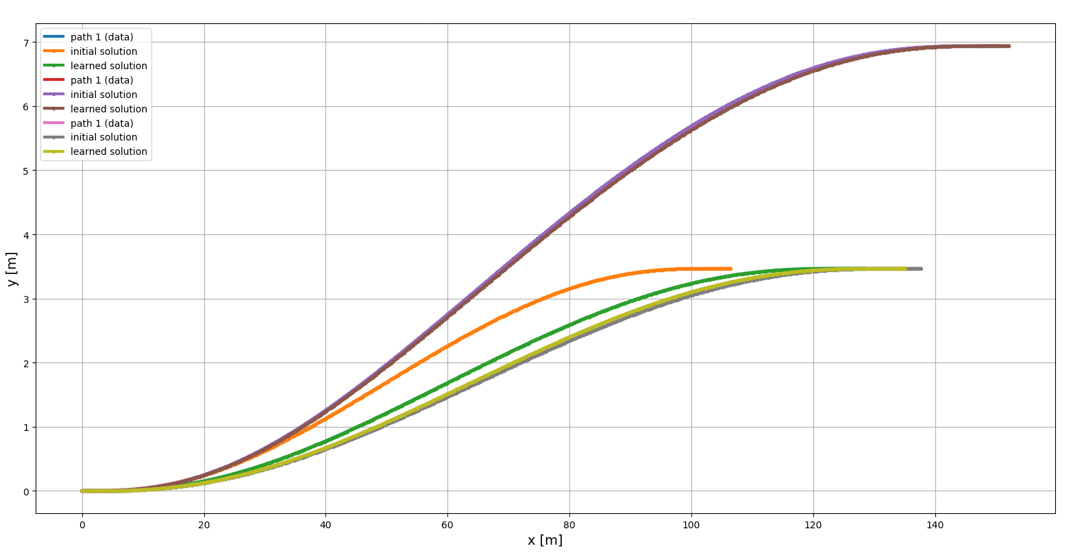
\includegraphics[width=1.0\textwidth]{result_seq.png}
	\caption{Overview of initial guesses, learned and observed trajectories.} 
	\label{fig:result_seq}
\end{figure}

\begin{figure}[h!]
	\centering
	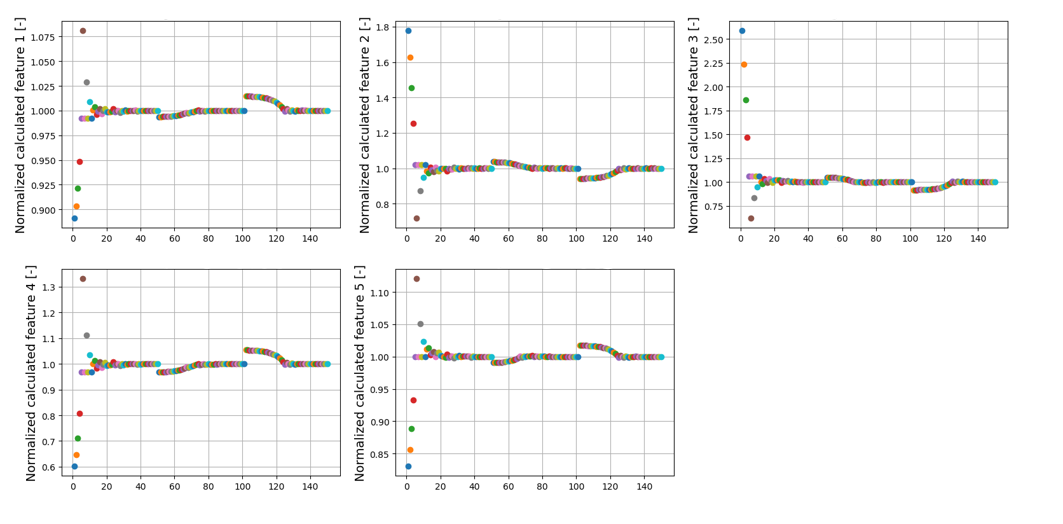
\includegraphics[width=1.2\textwidth]{convergence_seq.png}
	\caption{Convergence of the features with learned weights towards the observed features according to section \ref{s:obj}}
	\label{fig:convergence_seq}
\end{figure}

Convergence is attained after $50$, $51$ and $49$ iterations. From Figure \ref{fig:result_seq} it is clear that when features accurately match as visualized in Figure \ref{fig:convergence_seq}, the observed path is accurately reconstructed when using ideal observations. It can be concluded that fitting of the features gives a good reproduction of the individual state and control signals. Furthermore convergence is fast obtained because the amount of iterations stays limited and simulation time is under 5 minutes per dataset.\\

 An interesting result however is that the corresponding features are not found back. The learned weights are respectively $\bigl[ \begin{smallmatrix} 0.45  ,&1.44 ,&1.68 ,&0.39,&0.60\end{smallmatrix}\bigr]$, 
 
 $\bigl[ \begin{smallmatrix} 0.45  ,&1.48 ,&1.71 ,&0.35,&0.59\end{smallmatrix}\bigr]$ and $\bigl[ \begin{smallmatrix} 0.63  ,&1.43 ,&1.69 ,&0.37,&0.60\end{smallmatrix}\bigr]$. This is visualized in Figure \ref{fig:convergence_seq} by the small jump when switched to a different dataset. Figure \ref{fig:result_seq} shows in orange the first initial guess and in green the learned solution which matches the observed one in blue. The other generated paths start from a close but not perfect initial guess.\\
 
 For each different dataset features match exactly but this is not done for the exact same weights because local solutions exist that explain individual datasets. It should be noted that the relative sizes of the learned weights matches the original one except for the feature concerning longitudinal acceleration which don't play a dominant role during a lane change. \textbf{Question: how is this when you do an acceleration maneuver??}\\
 
 Next the influence of the numerical discretization is checked. A better discretization is obtained when a larger amount of optimization points $N$ is chosen which lead to a smaller time discretization $dt$, but comes at the cost of a higher computational load. Figure \ref{fig:N_influence} shows the error on the features discussed in section \ref{s:obj} when using the learned weights based on dataset A for predicting the observations of dataset B. The convergence criteria of the learned weights are set on $f_{rel,i}$ equal to $10^{-1}$. It is concluded that there is no large influence on the amount of optimization points chosen.\\
 
 \begin{figure}[h!]
 	\centering
 	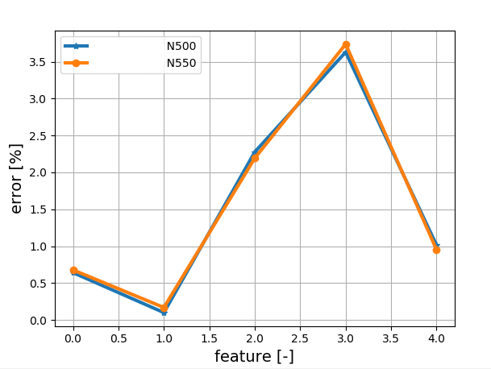
\includegraphics[width=0.7\textwidth]{N_influence.png}
 	\caption{Different error made when using a different amount of optimization points in \ref{opt:basic_opti_w}.}
 	\label{fig:N_influence}
 \end{figure}
 
 In order to further validate the learning algorithm, the chosen weights were given as initial guess making use of one dataset in order to check if it would diverge from the ideal global solution. As expected the algorithm converged after the first iteration. Next a guess close to the global solution was tried. The algorithm converged after $41$ iterations and outputted $\bigl[ \begin{smallmatrix} 4.01,&5.29,&6.33,&1.09,&2.12\end{smallmatrix}\bigr]$ and not $\bigl[ \begin{smallmatrix} 4.0,&5.0,&6.0,&1.0,&2.0\end{smallmatrix}\bigr]$ which proofs that a lot of local solutions exist.\\  
 
 From above tests it can be concluded that the local solutions of individual datasets do not match and that the amount of mismatch has only a small dependants on the amount of optimization points. The next step to take is to combine different datasets in simultaneous learning instead of sequential learning in order to try to converge to weights that predict best for multiple datasets. 
 
 \subsection{Conflict method}
 The first method proposed is the conflict method. Is main idea is to update the weights in the common direction of the gradient seen in equation \ref{eq:new} of the different datasets. If the direction of update according to gradient method is conflicting between different datasets the update of the weight in question is put on hold. The updating will be resumed when the conflict is resolved by updating the other weights. This is possible because the features are not independent of each other. Figure \ref{fig:conflict} shows how the conflict method will be embedded in the basic flow of the learning algorithm.\\
 
  \begin{figure}[h!]
 	\centering
 	\includegraphics[width=1.1\textwidth]{conflict.png}
 	\caption{Flow of the conflict method as part of the basic flow diagram of Figure \ref{fig:basic learning}}
 	\label{fig:conflict}
 \end{figure}

Depending if the previous case in the RPROP algorithm was case 2 and the sign difference between the current and previous gradient, three distinct RPROP cases can be identified with other update methods as discussed in section \ref{s:RPROP}. Inside the conflict test, it is checked if all the signs of the current gradients of the different datasets are checked. If there is a sign difference, this means that for one dataset a feature value is higher than the observed one and the corresponding weight should be increased (negative gradient) and for an other dataset it is the other way around and the corresponding weight should be decreased. (positive gradient). For such a case the conflict test will give rise to a positive conflict value. If there is no conflict there will also be unity in the decision of the RPROP case. After the conflict is solved, the next case will be automatically equal to case 3 because no decision can be made about the increase or decrease of the update value. The convergence criteria used is aside of the maximum amount of iterations and an accurate match of $10^{-4}$ with the observed features the criteria if there is still improvement possible in a direction that benefits every dataset.\\

The learning algorithm is applied simultaneously to dataset A,B and C and uses as initial guess for the weights the vector $\bigl[ \begin{smallmatrix} 1.0,&1.0,&1.0,&1.0,&1.0\end{smallmatrix}\bigr]$. The algorithm is ended after $17$ iterations with no direction of improvement possible. The observed paths with their initial guesses and learned paths can be seen in Figure \ref{fig:conflict_paths}.

 
 \begin{figure}[h!]
 	\centering
 	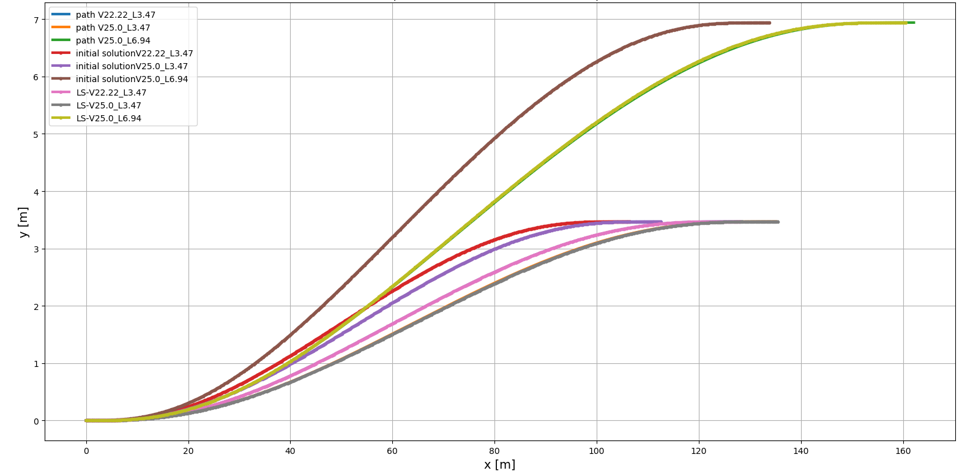
\includegraphics[width=1.0\textwidth]{conflict_path.png}
 	\caption{Overview of the different observed paths, initial guesses and learned paths.}
 	\label{fig:conflict_paths}
 \end{figure}

The convergence plots are all similar and for dataset A, Figure \ref{fig:conflict_convergence}, gives the convergence of $f_{rel,i}$ for the different features. 
 \begin{figure}[h!]
	\centering
	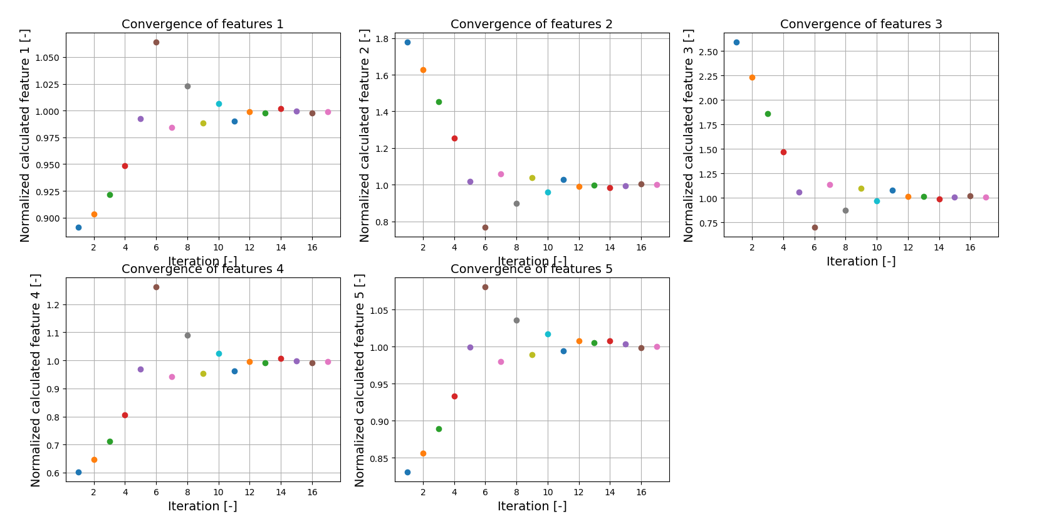
\includegraphics[width=1.15\textwidth]{conflict_convergence.png}
	\caption{Convergence plot of $f_{rel,i}$ for dataset A.}
	\label{fig:conflict_convergence}
\end{figure}
 
 As is indicated by Figure \ref{fig:conflict_convergence}, the method is clearly converging towards the different sets of observed feature vectors. However it should be noted that despite giving more accurate results for the feature values of the other datasets then when only one dataset A is used to learn the weights, the method is still constricted in its feature matching accuracy due to no available direction of improvement. This effect worsens when more datasets are used because conflicts more rapidly occur. Table \ref{table:conflict_weights} lists the different learned weights and Figure \ref{fig:conflict_accuracy} shows the loss of accuracy when more datasets are simultaneously learned.
 
 

\begin{figure}[h!]
	\centering
	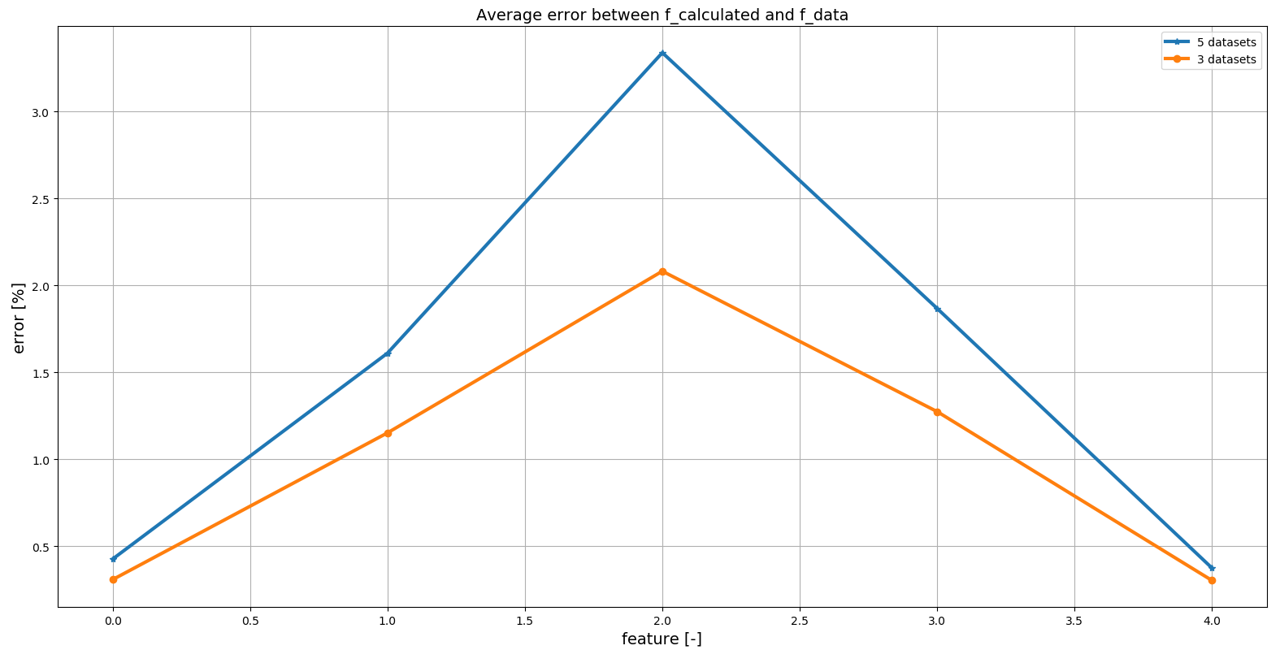
\includegraphics[width=1.0\textwidth]{conflict_accuracy.png}
	\caption{The average error between the observed and calculated feature values with the learned weights when applying the conflict method.}
	\label{fig:conflict_accuracy}
\end{figure}

 \subsection{Averaging method}
 In this method not all the different observed feature vectors are taken individually into account when updating the weights, but a single averaged observed feature vector is used. This avoids conflicting local solution. The flow of the algorithm is thus similar as shown in Figure \ref{fig:basic learning} but instead of a single dataset an averaged is used. In order to calculate the gradient, the difference between the averaged observed feature vector and the averaged calculated feature vector has to be taken. In order to obtain the averaged calculated feature vector, m times the optimization \ref{opt:basic_opti_w} is called for each specific observed maneuver. Afterwards the individual found feature vectors are averaged. With m the amount of observed datasets. This method is based on \cite{Kuderer2015a}.\\
 
% Bespreek de fixed feature approach.

 The learning of the three datasets A,B and C is done with as stop criteria the maximum amount of iterations and convergence towards the averaged feature values with an accuracy of $10^{-4}$. The initial guess chosen for the weights is an all one vector. Convergence is reached after $111$ iterations because the desired convergence accuracy is reached. The learned weights are $\bigl[ \begin{smallmatrix} 1.21,&1.53,&1.83,&0.31,&0.61\end{smallmatrix}\bigr]$. 
 

 
 \subsection{Comparison of methods}
 In this section a comparison is made between the average and conflict method of combining different datasets. 
 
 \begin{table}[h!]
 	\centering
 	\begin{tabular}{@{}llr@{}} 
 		Weight    & Average & Conflict\\ \midrule
 		Nr.2      & \hspace{7mm}0.0    & 0.0 \\
 		Nr.4      & \hspace{7mm} 0.0074    & 0.032 \\
 		Nr.6      & \hspace{7mm}0.0029    & 0.00045 \\ \bottomrule
 	\end{tabular}
 	\caption{The error made between the learned and chosen weights for respectively the average and conflict method.}
 	\label{table:error_learned_weights_conflict}
 \end{table}

  , 
 \subsection{Conclusion}


%algorithm zelf%
% normalization% 
% data generation%
% discussion and conclusion of single dataset learning --> lot of local solutions
% --> numerical assessment
% methods for multiple datasets
% initial values, things that are varied --> width of the road and initial longitudinal speed.
% Other maneuvers --> acceleration
% Bekijk slides!


%%%%%%%%%%%%%%%%%%%%%%%%%%%%%
%\textbf{Discussion of the algorithm of the lane change}
% In the first constraint in algorithm \ref{alg:1} the path closing constraints are put into the algorithm. In the initialization constraint, the first states are set equal to the condition of the system at the start of the lane change. In this report all states are assumed equal to zero at the start of the lane change except for the longitudinal velocity. In the end constraint the desired final condition of the system is specified. That is, the vehicle has done a lane change and is driving straight again.\\

%De gevonden trajectories vergelijken met een standaard lane change uit de literatuur --> zie $lane_change_kin$ voor foto. \\
%
%Hoe is algorithm opgebouwd? Wrm wordt dit zo gedaan?
%Welke vehicle modellen wordt er gebruikt? Wrm mag men hier een simple vehicle mode gebruiken?
%Dit is gemachtigd omdat men hier de omgeving wil scannen voor een feasible pad --> dit wordt trager gedaan dan de tracking.(tracking zal gebruik maken van een meer complex model) Path planning ligt focus vooral op de omgeving.
%Hoe zal de methode gevalideerd worden? Leg de twee methodes uit: code generatie en kijken of de wegings factoren terug gevonden kunnen worden? Mappen de feature values met de values van het geobserveerde pad? --> is het doel dat gevolgd probeert te worden haalbaar? 

%Vermeld afleiding van algortihm. Leg uit in Thesis hoe komt aan gradient die gebruikt. Zie papers: Ziebart et al and Kretzschmar et al.
%
%Modeleer een andere bestuurder. Can try to reproduce a data set with a change of parameters which represents a different driver. Can check that the learned model is also different. Hiermee aantonen dat er ook echt andere wegingsfactoren worden gegenereerd en dat de specifieke driving characteristics worden meegenomen.
%
%Ligt een tipje van de sluier op : hoe zal de data gegenereerd worden? 

%
%Maak een vermelding dat men het menselijke gedrag van het geleerde model kan nagaan met een Turing test.\\
%
%Maak een plotje zoals paper Learning to Predict Trajectories of Cooperatively Navigating Agents --> feature variance afwijking en average error. (zelfde plotjes als al de papers)\\
%
%Schrijf een paragraaf over hoe de data gegenereerd wordt. %
%
%Kan vermelding maken dat in deze thesis de features zijn gekozen met de hand --> men kan proberen om de features ook te leren van date (Characterizing Driving Styles with Deep Learning)
% Try to validate the chosen features with looking at the sensitivity.

%%Afleiding van exponentiël functie zie paper: Feature-based prediction of trajectories for socially compliant navigation (foto) --> weights are lagrange coefficients.


%\section{Tables}
%Tables are used to present data neatly arranged. A table is normally
%not a spreadsheet! Compare \tref{tab:wrong} en \tref{tab:ok}: which table do
%you prefer?
%
%\begin{table}
%  \centering
%  \begin{tabular}{||l|lr||} \hline
%    gnats     & gram      & \$13.65 \\ \cline{2-3}
%              & each      & .01 \\ \hline
%    gnu       & stuffed   & 92.50 \\ \cline{1-1} \cline{3-3}
%    emu       &           & 33.33 \\ \hline
%    armadillo & frozen    & 8.99 \\ \hline
%  \end{tabular}
%  \caption{A table with the wrong layout.}
%  \label{tab:wrong}
%\end{table}
%
%\begin{table}
%  \centering
%  \begin{tabular}{@{}llr@{}} \toprule
%    \multicolumn{2}{c}{Item} \\ \cmidrule(r){1-2}
%    Animal    & Description & Price (\$)\\ \midrule
%    Gnat      & per gram    & 13.65 \\
%              & each        & 0.01 \\
%    Gnu       & stuffed     & 92.50 \\
%    Emu       & stuffed     & 33.33 \\
%    Armadillo & frozen      & 8.99 \\ \bottomrule
%  \end{tabular}
%  \caption{A table with the correct layout.}
%  \label{tab:ok}
%\end{table}





%In order to implement the above defined first and second derivative and integrations in a CasADi optimization environment, discretization with a numerical scheme is needed. The first and second derivative are discretized by means of a central scheme as can be seen in equation \ref{eq:CC}


%\begin{subequations}
%	\begin{equation}
%	\pdv{\phi}{t} = \frac{\phi(i+1)-\phi(i-1)}{2\Delta t}
%	\end{equation}
%	\begin{equation}
%	\pdv[2]{\phi}{t} = \frac{\phi(i+1)\phi(i)+\phi(i-1)}{\Delta t^2}
%	\end{equation}
%\end{subequations}
%
%The Crank-Nicolson numerical integration as is displayed in equation \ref{eq:CN} is used in order to obtain the different feature values of feature $i$.
%\begin{subequations}\label{eq:CN}
%	\begin{equation}
%	\int_{f_i(t^n)}^{f_i(t^{n+1})}df_i=\int_{t^n}^{t^{n+1}} I(t) \cdot dt	
%	\end{equation}
%	\begin{equation}
%	f_i^{n+1} -f_i^{n} = \frac{1}{2}\frac{I(t^{n+1})+I(t^n)}{\Delta t}
%	\end{equation}
%\end{subequations}\\


%%% Local Variables: 
%%% mode: latex
%%% TeX-master: "thesis"
%%% End: 
